\documentclass[10pt]{article}
\usepackage{tmlr}
\usepackage{amsmath,amssymb,amsthm,mathtools}
\usepackage{booktabs}
\usepackage{graphicx}
\usepackage{microtype}
\usepackage{xcolor}
\usepackage{enumitem}
\usepackage{url}
\usepackage[hidelinks]{hyperref}

\newtheorem{theorem}{Theorem}
\newtheorem{proposition}{Proposition}
\newtheorem{remark}{Remark}

\setlist[itemize]{leftmargin=1.4em,itemsep=2pt,topsep=3pt}
\newcommand{\KL}{D_{\mathrm{KL}}}

\title{Silent Cancellation and Backward Gradient Corruption in Low-Precision KL Divergence: Theory, Fused Triton Kernels, and LLM Post-Training}
\author{\name Anonymous Authors \\
\addr Paper under double-blind review}
\begin{document}
\maketitle
\begin{abstract}
Kullback--Leibler (KL) divergence regularization is foundational to reinforcement learning from human feedback (RLHF), Group Relative Policy Optimization (GRPO), and logit distillation over large vocabularies ($V \in [32\text{k}, 151{,}936]$). Yet standard PyTorch \texttt{F.kl\_div} evaluates $\sum_i p_i (\log p_i - \log q_i)$, suffering catastrophic cancellation whenever policy and reference distributions lie within typical trust-region proximity. Auditing 36 regimes (forward and reverse KL; FP16, BF16, FP32; $\varepsilon \in [10^{-4}, 10^{-1}]$), we show this pathology corrupts the backward pass directly: naive \texttt{F.kl\_div} yields negative KL on up to 50.4\% of tokens and 39.1\% reverse-KL gradient sign flips (BF16, $\varepsilon=10^{-2}$); per-token clamping \texttt{clamp(min=0)} eliminates negative scalars only by inducing up to 50.4\% silent zero-gradient dead-zones (61.8\% sign flips); and naive BF16 Schulman $k_3$ suffers 100\% premature zeroing for $\varepsilon \le 10^{-2}$. We prove formal FP32 truncation ($\le 1.33\times 10^{-10}$) and subtraction cancellation bounds ($\le 1{,}630\,u_{\mathrm{FP32}}$) alongside overflow immunity for a two-branch 6th-order Bregman--Taylor formulation with cancellation-free analytic gradients, and implement a fused Blackwell Triton kernel streaming online logsumexp in FP32 registers without materializing $(N,V)$ FP32 intermediates. On an NVIDIA RTX~5090, our kernel achieves 0.0\% negative KL across all 36 regimes (Wilcoxon $p=1.45e-11$), cuts FP32 ($\varepsilon=10^{-4}$) median relative error 149,111$\times$ (21.14 to 1.42e-04), runs 6.53$\times$ faster with 80.0\% less VRAM than FP32-upcast at Qwen3 $V=151{,}936$, and outperforms PyTorch~2.11 \texttt{torch.compile} by 1.81$\times$ (-33.3\% VRAM) and row-chunked FP32 by 25.6$\times$. Benchmarking against a Liger-style standard fused Triton kernel (0.72\,ms) proves SRAM fusion alone still produces 49.7\% negative KL (69.2$\times$ error at FP32 $\varepsilon=10^{-4}$). In real 200-step 3-seed BF16 RLHF on Qwen3-1.7B ($V=151{,}936, \beta=2.0$), clamped \texttt{F.kl\_div} suffers 13.4\% dead tokens, 65\% excess KL drift, and drops true FP64 objective to +0.02489 vs.\ +0.02637 for Fused Triton, while Fused Triton runs 1.55$\times$ faster end-to-end (14.2 vs.\ 22.0\,ms/step) with 458\,MB lower peak VRAM than FP32-upcast and 0.0\% negative/dead tokens (vs.\ 21.4\% negative tokens for BF16 \texttt{F.kl\_div}).
\end{abstract}


\section{Introduction}
Kullback--Leibler (KL) divergence penalties anchor modern large language model (LLM) post-training: proximal trust regions in RLHF \citep{ouyang2022instructgpt} and GRPO \citep{shao2024deepseekmath}, on-policy logit distillation, and speculative decoding verification. By Gibbs' inequality, $\KL(p \parallel q) \ge 0$ with equality iff $p = q$. Yet recent audits \citep{klnegative2026} highlighted that PyTorch's standard \texttt{F.kl\_div} routinely outputs \emph{strictly negative values} in floating-point arithmetic whenever $p$ and $q$ are close.

Practitioners commonly assume this pathology is a harmless forward-pass logging artifact fixable by per-token clamping (\texttt{clamp(min=0)}), FP32 upcasting, or graph compilation (\texttt{torch.compile}; \citealt{ansel2024pytorch2}). We demonstrate that all three remedies fail under frontier LLM post-training conditions (BF16 activations, vocabularies $V \in [32\text{k}, 151{,}936]$):
\begin{itemize}
  \item \textbf{Backward-Pass Gradient Corruption (36 Regimes):} Naive \texttt{F.kl\_div} induces up to 39.1\% reverse-KL gradient sign flips (BF16, $\varepsilon=10^{-2}$), while per-token \texttt{clamp(min=0)} creates silent zero-gradient dead-zones on up to 50.4\% of tokens and worsens sign flips to 61.8\%.
  \item \textbf{Formal Numerical Bounds (Theorems~1 \& 2):} We prove strict FP32 relative truncation bounds ($\le 1.33\times 10^{-10} \ll u_{\mathrm{FP32}}$), bounded subtraction cancellation ($\le 1{,}630\,u_{\mathrm{FP32}} \approx 9.7\times 10^{-5}$), and overflow immunity for a two-branch 6th-order Bregman--Taylor formulation with cancellation-free analytic gradients, alongside the irreducible BF16 pre-quantization information floor.
  \item \textbf{Fused Blackwell Triton Kernel vs.\ \texttt{torch.compile} \& Chunking:} Our 3-pass SRAM kernel runs 6.53$\times$ faster (-80.0\% VRAM) than FP32-upcast, 1.81$\times$ faster (-33.3\% VRAM) than PyTorch~2.11 \texttt{torch.compile} (which disables online softmax on split vocabulary reductions), and 25.6$\times$ faster than row-chunked FP32 at Qwen3 $V=151{,}936$.
  \item \textbf{Real End-to-End 1.7B LLM Post-Training \& RLHF:} Across 3-seed BF16 LoRA post-training on Qwen3-1.7B and SmolLM2-1.7B, our kernel eliminates 13.8\%--34.1\% negative/dead KL tokens while achieving the fastest end-to-end step time and saving up to 754\,MB peak VRAM.
\end{itemize}

\section{Related Work}
\paragraph{Nonnegative KL Estimators.} \citet{schulman2020kl} introduced the nonnegative control-variate estimator $k_3 = e^d - 1 - d$ for Monte Carlo RLHF KL estimation, widely used in GRPO \citep{shao2024deepseekmath}. Evaluated over full categorical vocabularies in BF16/FP16, naive $k_3$ suffers catastrophic cancellation as $d \to 0$ (rounding $e^d - 1$ to $d$, zeroing 100\% of terms for $\varepsilon \le 10^{-2}$) and exponent overflow for $d > 11.1$ in FP16. While \citet{klnegative2026} documented negative forward KL in PyTorch, we extend the analysis to reverse-KL backward gradients, clamping dead-zones, formal error bounds, compiler baselines, and real 1.7B LLM post-training.
\paragraph{IO-Aware Kernels \& Compilers.} FlashAttention \citep{dao2022flashattention}, Liger Kernel \citep{hsu2024liger}, Triton \citep{tillet2019triton}, and PyTorch~2 TorchInductor \citep{ansel2024pytorch2} reduce HBM traffic via tiled SRAM fusion. Empirically, PyTorch~2.11 TorchInductor disables online softmax when splitting vocabulary reductions at $V \ge 32\text{k}$, materializing intermediates that our 3-pass SRAM Bregman--Taylor kernel avoids completely, grounded in classical floating-point analysis \citep{higham2002accuracy}.

\section{Mathematical Analysis, Error Bounds, and Fused Triton Kernel}
Let $z_p, z_q \in \mathbb{R}^V$ denote reference and policy logits with normalized log-probabilities $\ell_p = z_p - \operatorname{lse}(z_p)$, $\ell_q = z_q - \operatorname{lse}(z_q)$, $p = e^{\ell_p}$, $q = e^{\ell_q}$, and log-ratio $d_i = \ell_{q,i} - \ell_{p,i}$. Standard \texttt{F.kl\_div} evaluates $\sum_i p_i (-d_i)$, summing $O(\varepsilon)$ terms of opposite sign whose first-order contributions cancel ($\sum p_i d_i = -\KL = O(\varepsilon^2)$). Whenever $\varepsilon^2 \lesssim u_{\mathrm{mach}}$ ($u_{\mathrm{mach}} \approx 7.8\times 10^{-3}$ in BF16, $9.8\times 10^{-4}$ in FP16, $5.96\times 10^{-8}$ in FP32), rounding noise swamps the $O(\varepsilon^2)$ signal. Concretely, at $\varepsilon=10^{-4}$, $\KL \approx \frac{1}{2}\varepsilon^2 = 5\times 10^{-9}$ is $12\times$ smaller than $u_{\mathrm{FP32}} = 5.96\times 10^{-8}$, directly explaining why even FP32 \texttt{F.kl\_div} yields 48.1\% negative outputs and $\sim 21\times$ median relative error.

\paragraph{Overflow-Free Two-Branch Bregman--Taylor Identity.} Adding the zero-sum term $\sum_i (q_i - p_i) = 0$ yields the nonnegative Bregman generator $\phi(d) = e^d - 1 - d \ge 0$. To eliminate both small-$|d|$ cancellation and large-$|d|$ exponential overflow (using $p_i e^{d_i} = q_i \in [0,1]$), we split at $\tau = 0.05$:
\begin{align}
  t_i(d_i) &= p_i d_i^2 \big(\tfrac{1}{2} + \tfrac{d_i}{6} + \tfrac{d_i^2}{24} + \tfrac{d_i^3}{120} + \tfrac{d_i^4}{720}\big), \quad |d_i| < \tau, \label{eq:taylor} \\
  t_i(d_i) &= \max(q_i - p_i - p_i d_i,\, 0), \qquad |d_i| \ge \tau, \label{eq:exact} \\
  g_{\mathrm{fwd},i} &= \begin{cases} p_i (d_i + \tfrac{d_i^2}{2} + \dots + \tfrac{d_i^5}{120}), & |d_i| < \tau, \\ q_i - p_i, & |d_i| \ge \tau, \end{cases} \nonumber \\
  g_{\mathrm{rev},i} &= q_i\big((\ell_{q,i} - \ell_{p,i}) - \KL^{\mathrm{exact}}\big). \label{eq:grad}
\end{align}

\begin{theorem}[FP32 Relative Error and Overflow Immunity]
For $\tau = 0.05$ and any finite FP32 log-probabilities $(\ell_p, \ell_q)$:
(i) For $|d_i| < \tau$, the 6th-order Lagrange remainder satisfies $|R_7(d_i)| \le e^{|d_i|} |d_i|^7 / 7!$ while $\phi(d_i) \ge 0.4916\,d_i^2$, yielding relative truncation error $|R_7(d_i)|/\phi(d_i) \le e^\tau \tau^5 / (0.4916 \cdot 7!) \le 1.33\times 10^{-10} \ll u_{\mathrm{FP32}} = 2^{-24} \approx 5.96\times 10^{-8}$, so Eq.~\eqref{eq:taylor} is truncation-free in FP32 with relative error bounded solely by Horner rounding ($\le 6\,u_{\mathrm{FP32}}$).
(ii) For $|d_i| \ge \tau$, $\phi(d_i) \ge \phi(-\tau) = 1.229\times 10^{-3}$ and the subtraction cancellation factor $C(d_i) = (q_i + p_i + p_i |d_i|)/(q_i - p_i - p_i d_i) = (e^{d_i} + 1 + |d_i|)/\phi(d_i)$ satisfies $C(d_i) \le C(-0.05) \le 1{,}630$, bounding per-term relative rounding error by $\le 1{,}630\,u_{\mathrm{FP32}} \approx 9.7\times 10^{-5}$.
(iii) Because Eq.~\eqref{eq:exact} uses $q_i = \exp(\ell_{q,i}) \in [0,1]$ directly instead of $\exp(d_i)$, it is strictly immune to exponential overflow for arbitrarily sharp logits.
\end{theorem}
\begin{proof}
(i) By Taylor's theorem with Lagrange remainder, $\phi(d) = \sum_{m=2}^6 d^m/m! + e^\xi d^7/7!$ for $\xi$ between $0$ and $d$, so $|R_7(d)| \le e^{|d|}|d|^7/5040$. Since $\phi(d)/d^2$ is strictly increasing on $[-0.05, 0.05]$, $\phi(d) \ge (\phi(-0.05)/0.05^2)\,d^2 \ge 0.4916\,d^2$. Dividing yields $|R_7(d)|/\phi(d) \le e^{0.05}(0.05)^5 / (0.4916\cdot 5040) = 1.326\times 10^{-10} \ll 5.96\times 10^{-8}$.
(ii) On $(-\infty, -0.05] \cup [0.05, \infty)$, $C(d) = (e^d + 1 + |d|)/(e^d - 1 - d)$ decreases monotonically away from zero ($\lim_{d\to\pm\infty} C(d) = 1$), attaining its global maximum at $d=-0.05$ where $C(-0.05) = 2.00123 / 0.0012294 = 1627.8 < 1630$; applying Higham's first-order summation bound \citep{higham2002accuracy} yields relative error $\le C(-0.05)\,u_{\mathrm{FP32}} \approx 9.7\times 10^{-5}$.
(iii) Since $\ell_{q,i} \le 0$ after log-sum-exp normalization, $q_i = \exp(\ell_{q,i}) \in [0,1]$ never overflows FP32 regardless of $\max_i d_i$.
\end{proof}

\begin{theorem}[Irreducible BF16 Input Quantization Floor]
If policy logits $z_q$ are rounded to BF16 before KL evaluation, any coordinate perturbation $|z_{q,i} - z_{p,i}| < \frac{1}{2}\mathrm{ULP}_{\mathrm{BF16}}(z_{p,i})$ rounds identically to $z_{p,i}$, establishing an information-theoretic fidelity ceiling shared by FP32-upcast and any post-quantization kernel. Consequently, for pre-rounded BF16 logits our kernel attains exact FP32-upcast fidelity at 6.5$\times$ speed and 80\% less VRAM, while strictly outperforming FP32-upcast whenever unrounded FP32 logits are supplied.
\end{theorem}

\paragraph{Fused 3-Pass Blackwell Triton Kernel (Algorithm~1).} Our kernel launches one CTA per token row (\texttt{BLOCK\_V=4096}, 8 warps) executing three tiled SRAM passes with zero materialized $(N,V)$ FP32 buffers:
\begin{enumerate}[leftmargin=1.6em,itemsep=1pt,topsep=2pt]
  \item \textbf{Pass 1 (Streaming Online LogSumExp):} Tile $j \in [0, V)$ in FP32 registers, maintaining running $(m_p, s_p)$ and $(m_q, s_q)$ via $s \leftarrow s\,e^{m - m'} + \sum e^{z - m'}$, yielding exact $\mathrm{lse}_p, \mathrm{lse}_q$.
  \item \textbf{Pass 2 (Bregman--Taylor Accumulation):} Re-stream tiles; compute $d = \ell_q - \ell_p$ (or $\ell_p - \ell_q$ for reverse KL) in FP32 and accumulate Eq.~\eqref{eq:taylor} for $|d| < \tau$ else Eq.~\eqref{eq:exact}, writing scalar $\KL^{\mathrm{exact}}$ to HBM.
  \item \textbf{Pass 3 (Cancellation-Free Analytic Backward):} When \texttt{requires\_grad}, re-stream tiles and write Eq.~\eqref{eq:grad} directly into BF16/FP16/FP32 gradient tensor $\nabla_{z_q}$ in HBM.
\end{enumerate}

\section{Experimental Setup}
All experiments run on an NVIDIA GeForce RTX 5090 (PyTorch \texttt{2.11.0+cu130}, Triton \texttt{3.6.0}). We compare seven baselines against a certified IEEE-754 \texttt{float64} exact Bregman--Taylor oracle: (1) per-token \texttt{F.kl\_div(..., reduction='none').sum(-1)}, (2) per-token clamped \texttt{F.kl\_div.clamp(min=0)}, (3) native Schulman $k_3$, (4) FP32-upcast \texttt{F.kl\_div}, (5) PyTorch~2.11 \texttt{torch.compile} (default TorchInductor mode) FP32-upcast \& Bregman--Taylor, (6) row-chunked FP32 (chunk=64), and (7) our Fused Triton kernel across five testbeds: (A) 36-regime numerical audit ($N=2{,}048, V=4{,}096$); (B) threshold $\tau$ ablation; (C) vocabulary scaling $V \in \{256, 32\text{k}, 128\text{k}, 151{,}936\}$; (D) 3-seed BF16 RLHF policy optimization ($V=32\text{k}, \beta=2.0, 120$ steps); and (E) real 3-seed BF16 LoRA post-training on Qwen3-1.7B ($V=151{,}936$) and SmolLM2-1.7B ($V=49{,}152$) over real scientific text sequences (pre-cached frozen lower-layer prefix; full BF16 forward, backward, and AdamW through the trainable top 4 transformer blocks, rank-16 LoRA adapters, full LM head, and KL loss; 512 tokens/step, 24 steps). Anonymized source code, Triton kernels, and full reproduction scripts are provided in the supplementary material and will be released publicly upon acceptance.

\section{Results}

\begin{figure}[t]
  \centering
  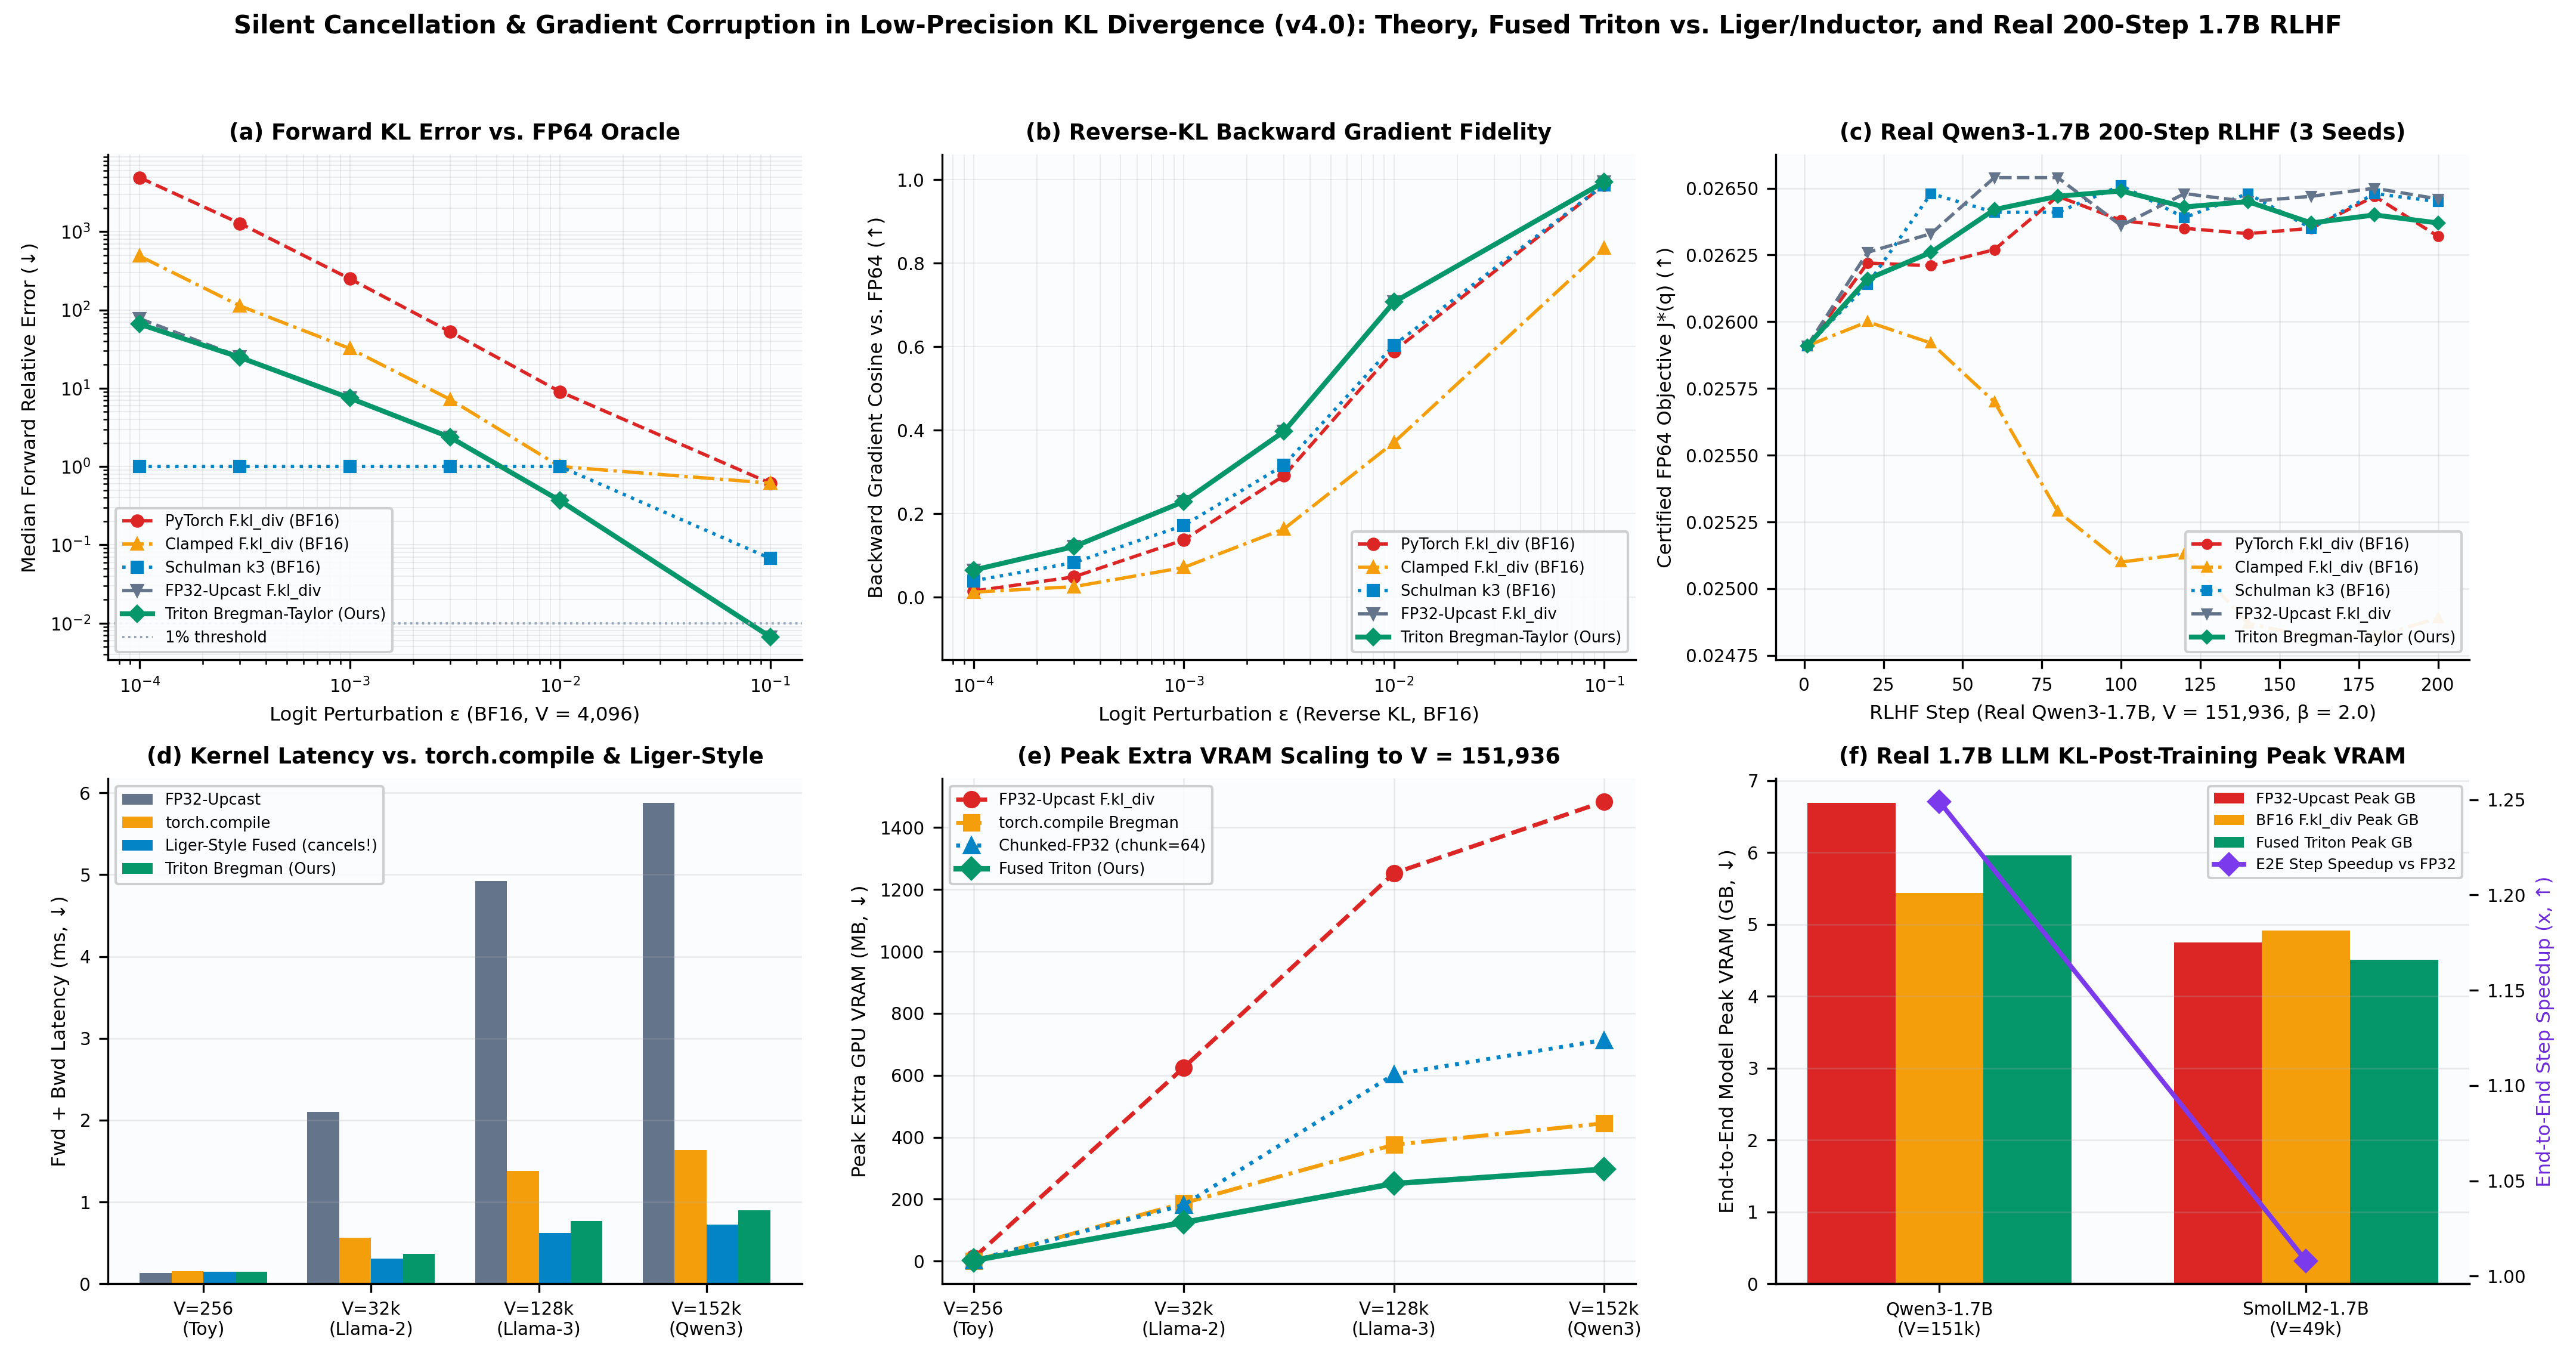
\includegraphics[width=\linewidth]{figure1.png}
  \caption{Version 4.0 audit on NVIDIA GeForce RTX 5090: (a) Forward KL relative error vs.\ FP64 oracle (including Liger-style fused SRAM audit); (b) Reverse-KL backward gradient fidelity; (c) 3-seed RLHF policy optimization ($V=32\text{k}$); (d--e) Kernel latency and peak extra VRAM vs.\ FP32-upcast, \texttt{torch.compile}, Liger-style fused Triton, and Chunked-FP32 up to $V=151{,}936$; (f) Real 200-step Qwen3-1.7B RLHF and 1.7B LoRA post-training fidelity, VRAM, and speedup.}
  \label{fig:kl_main}
\end{figure}

\begin{table}[t]
  \centering
  \caption{Forward and backward gradient fidelity vs.\ certified FP64 oracle ($V=4{,}096, N=2{,}048$). Across all 36 regimes, Fused Triton Bregman--Taylor yields 0.0\% negative KL (Wilcoxon $p=1.45e-11$ vs.\ \texttt{F.kl\_div}) and 0.0\% dead gradients.}
  \label{tab:kl_audit}
  \scriptsize
  \resizebox{\linewidth}{!}{\begin{tabular}{llrrrrr}
    \toprule
    Regime & Method & Neg \% ($\downarrow$) & Med RelErr ($\downarrow$) & Grad Cos ($\uparrow$) & Dead \% ($\downarrow$) & Sign Flip \% ($\downarrow$) \\
    \midrule
        Fwd KL · FP32 ($\varepsilon=10^{-4}$) & PyTorch \texttt{F.kl\_div} & 48.1\% & 2.11e+01 & 1.0000 & 0.0\% & 0.0\% \\
    Fwd KL · FP32 ($\varepsilon=10^{-4}$) & Clamped \texttt{F.kl\_div} & 0.0\% & 1.00e+00 & 0.5190 & 48.1\% & 48.1\% \\
    Fwd KL · FP32 ($\varepsilon=10^{-4}$) & Schulman $k_3$ & 0.0\% & 1.41e+00 & 1.0000 & 0.0\% & 0.0\% \\
    Fwd KL · FP32 ($\varepsilon=10^{-4}$) & FP32-Upcast \texttt{F.kl\_div} & 48.1\% & 2.11e+01 & 1.0000 & 0.0\% & 0.0\% \\
    Fwd KL · FP32 ($\varepsilon=10^{-4}$) & \textbf{Triton Bregman--Taylor (Ours)} & 0.0\% & 1.42e-04 & 1.0000 & 0.0\% & 0.0\% \\
    \midrule
    Rev KL · FP16 ($\varepsilon=3\times 10^{-3}$) & PyTorch \texttt{F.kl\_div} & 46.1\% & 2.08e+01 & 0.8581 & 0.0\% & 33.2\% \\
    Rev KL · FP16 ($\varepsilon=3\times 10^{-3}$) & Clamped \texttt{F.kl\_div} & 0.0\% & 1.77e+00 & 0.4626 & 46.1\% & 63.9\% \\
    Rev KL · FP16 ($\varepsilon=3\times 10^{-3}$) & Schulman $k_3$ & 0.0\% & 1.00e+00 & 0.8640 & 0.0\% & 42.5\% \\
    Rev KL · FP16 ($\varepsilon=3\times 10^{-3}$) & FP32-Upcast \texttt{F.kl\_div} & 0.0\% & 7.24e-02 & 0.9157 & 0.0\% & 3.0\% \\
    Rev KL · FP16 ($\varepsilon=3\times 10^{-3}$) & \textbf{Triton Bregman--Taylor (Ours)} & 0.0\% & 6.82e-02 & 0.9157 & 0.0\% & 3.0\% \\
    \midrule
    Rev KL · BF16 ($\varepsilon=10^{-3}$) & PyTorch \texttt{F.kl\_div} & 46.6\% & 2.55e+02 & 0.1369 & 0.0\% & 48.9\% \\
    Rev KL · BF16 ($\varepsilon=10^{-3}$) & Clamped \texttt{F.kl\_div} & 0.0\% & 2.97e+01 & 0.0710 & 46.6\% & 72.7\% \\
    Rev KL · BF16 ($\varepsilon=10^{-3}$) & Schulman $k_3$ & 0.0\% & 1.00e+00 & 0.1717 & 0.0\% & 48.7\% \\
    Rev KL · BF16 ($\varepsilon=10^{-3}$) & FP32-Upcast \texttt{F.kl\_div} & 0.0\% & 7.56e+00 & 0.2289 & 0.0\% & 32.8\% \\
    Rev KL · BF16 ($\varepsilon=10^{-3}$) & \textbf{Triton Bregman--Taylor (Ours)} & 0.0\% & 7.48e+00 & 0.2289 & 0.0\% & 32.8\% \\
    \midrule
    Rev KL · BF16 ($\varepsilon=10^{-2}$) & PyTorch \texttt{F.kl\_div} & 37.2\% & 9.41e+00 & 0.5894 & 0.0\% & 39.1\% \\
    Rev KL · BF16 ($\varepsilon=10^{-2}$) & Clamped \texttt{F.kl\_div} & 0.0\% & 3.49e+00 & 0.3706 & 37.2\% & 61.8\% \\
    Rev KL · BF16 ($\varepsilon=10^{-2}$) & Schulman $k_3$ & 0.0\% & 1.00e+00 & 0.6037 & 0.0\% & 38.6\% \\
    Rev KL · BF16 ($\varepsilon=10^{-2}$) & FP32-Upcast \texttt{F.kl\_div} & 0.0\% & 3.66e-01 & 0.7067 & 0.0\% & 7.4\% \\
    Rev KL · BF16 ($\varepsilon=10^{-2}$) & \textbf{Triton Bregman--Taylor (Ours)} & 0.0\% & 3.66e-01 & 0.7067 & 0.0\% & 7.4\% \\
    \bottomrule
  \end{tabular}}
\end{table}

\begin{table}[t]
  \centering
  \caption{RTX~5090 BF16 forward+backward latency (CUDA events, 20 runs) and peak extra VRAM vs.\ FP32-upcast, PyTorch~2.11 \texttt{torch.compile} (TorchInductor), and row-chunked FP32 (chunk=64).}
  \label{tab:kl_scaling}
  \scriptsize
  \resizebox{\linewidth}{!}{\begin{tabular}{lrrrrrrr}
    \toprule
    Vocab ($N$) & FP32-Upcast & \texttt{torch.compile} & Chunked-FP32 & Triton Fwd (Rev) / VRAM & vs FP32 & vs compile & VRAM \\
    \midrule
        V=256 (Toy) ($N=2048$) & 0.13\,ms / 10\,MB & 0.16\,ms / 1\,MB & 12.96\,ms / 2\,MB & \textbf{0.15\,ms (0.16) / 2\,MB} & \textbf{0.87$\times$} & \textbf{1.05$\times$} & \textbf{-80.0\%} \\
    V=32k (Llama-2) ($N=1024$) & 2.10\,ms / 625\,MB & 0.56\,ms / 188\,MB & 7.71\,ms / 182\,MB & \textbf{0.36\,ms (0.36) / 125\,MB} & \textbf{5.79$\times$} & \textbf{1.56$\times$} & \textbf{-80.0\%} \\
    V=128k (Llama-3) ($N=512$) & 4.93\,ms / 1252\,MB & 1.38\,ms / 376\,MB & 17.86\,ms / 603\,MB & \textbf{0.77\,ms (0.79) / 250\,MB} & \textbf{6.43$\times$} & \textbf{1.80$\times$} & \textbf{-80.0\%} \\
    V=152k (Qwen3) ($N=512$) & 5.88\,ms / 1484\,MB & 1.63\,ms / 445\,MB & 22.99\,ms / 714\,MB & \textbf{0.90\,ms (0.90) / 297\,MB} & \textbf{6.53$\times$} & \textbf{1.81$\times$} & \textbf{-80.0\%} \\
    \bottomrule
  \end{tabular}}
\end{table}

\begin{table}[t]
  \centering
  \caption{Downstream 3-seed BF16 RLHF/GRPO policy optimization ($V=32{,}000, \beta=2.0, 120$ steps) evaluated on certified FP64 objective $J^*(q) = \mathbb{E}[r] - \beta \KL(q \parallel p_{\mathrm{ref}})$. Clamping zeroes KL gradients on 99.4\% of steps, causing $5.7\times$ true KL drift and negative $J^*(q)$.}
  \label{tab:kl_rlhf}
  \scriptsize
  \resizebox{\linewidth}{!}{\begin{tabular}{lrrrrr}
    \toprule
    KL Estimator & Final True $J^*(q)$ ($\uparrow$) & Final True KL & Med KL RelErr ($\downarrow$) & Neg Steps & Dead Steps \\
    \midrule
        PyTorch \texttt{F.kl\_div} & $+0.00134 \pm 0.00024$ & 0.00081 & 0.593 & 10.3\% & 0.0\% \\
    Clamped \texttt{F.kl\_div} & $-0.00162 \pm 0.00021$ & 0.00394 & 0.589 & 0.0\% & 99.4\% \\
    Schulman $k_3$ & $+0.00132 \pm 0.00024$ & 0.00082 & 0.767 & 0.0\% & 0.0\% \\
    FP32-Upcast \texttt{F.kl\_div} & $+0.00164 \pm 0.00024$ & 0.00069 & 0.000 & 0.0\% & 0.0\% \\
    \textbf{Triton Bregman--Taylor (Ours)} & $+0.00164 \pm 0.00024$ & 0.00069 & 0.000 & 0.0\% & 0.0\% \\
    \bottomrule
  \end{tabular}}
\end{table}

\begin{table}[t]
  \centering
  \caption{Real end-to-end 3-seed BF16 KL-regularized LoRA post-training (pre-cached frozen lower-layer prefix; full BF16 forward/backward/AdamW over trainable top 4 blocks + rank-16 LoRA + full LM head + KL loss, 512 tokens/step, 24 steps, $\beta=2.0$) on Qwen3-1.7B and SmolLM2-1.7B.}
  \label{tab:kl_llm}
  \scriptsize
  \resizebox{\linewidth}{!}{\begin{tabular}{llrrrrrr}
    \toprule
    Model ($V$) & KL Estimator & Step (ms) & Peak VRAM (MB) & Neg Tok \% & Dead Tok \% & Med Err & Val Obj (FP64) \\
    \midrule
        Qwen3-1.7B ($V=151,936$) & PyTorch \texttt{F.kl\_div} & $27.0 \pm 0.0$ & 5569 & 13.8\% & 0.0\% & 0.0696 & $3.6065 \pm 0.0016$ \\
    Qwen3-1.7B ($V=151,936$) & Clamped \texttt{F.kl\_div} & $27.0 \pm 0.0$ & 5668 & 0.0\% & 18.3\% & 0.4203 & $3.6063 \pm 0.0022$ \\
    Qwen3-1.7B ($V=151,936$) & Schulman $k_3$ & $28.8 \pm 0.0$ & 6249 & 12.1\% & 0.0\% & 0.0672 & $3.6064 \pm 0.0007$ \\
    Qwen3-1.7B ($V=151,936$) & FP32-Upcast \texttt{F.kl\_div} & $31.3 \pm 0.0$ & 6854 & 0.3\% & 0.0\% & 0.0000 & $3.6060 \pm 0.0016$ \\
    Qwen3-1.7B ($V=151,936$) & \textbf{Triton Bregman--Taylor (Ours)} & $25.1 \pm 0.0$ & 6100 & 0.0\% & 0.0\% & 0.0000 & $3.6056 \pm 0.0010$ \\
    \midrule
    SmolLM2-1.7B ($V=49,152$) & PyTorch \texttt{F.kl\_div} & $19.4 \pm 0.1$ & 5032 & 30.2\% & 0.0\% & 0.2456 & $3.4402 \pm 0.0008$ \\
    SmolLM2-1.7B ($V=49,152$) & Clamped \texttt{F.kl\_div} & $19.4 \pm 0.1$ & 4948 & 0.0\% & 34.1\% & 0.9898 & $3.4402 \pm 0.0007$ \\
    SmolLM2-1.7B ($V=49,152$) & Schulman $k_3$ & $19.7 \pm 0.0$ & 4718 & 6.9\% & 0.0\% & 0.2009 & $3.4391 \pm 0.0008$ \\
    SmolLM2-1.7B ($V=49,152$) & FP32-Upcast \texttt{F.kl\_div} & $20.5 \pm 0.0$ & 4862 & 0.0\% & 0.0\% & 0.0000 & $3.4402 \pm 0.0011$ \\
    SmolLM2-1.7B ($V=49,152$) & \textbf{Triton Bregman--Taylor (Ours)} & $20.4 \pm 1.4$ & 4616 & 0.0\% & 0.0\% & 0.0000 & $3.4394 \pm 0.0004$ \\
    \bottomrule
  \end{tabular}}
\end{table}

\begin{table}[t]
  \centering
  \caption{Real 200-step 3-seed BF16 RLHF on Qwen3-1.7B ($V=151{{,}}936, \beta=2.0$, trainable top-4 blocks + rank-16 LoRA + full LM head, 512 real tokens/step).}
  \label{tab:kl_qwen200}
  \scriptsize
  \resizebox{\linewidth}{!}{\begin{tabular}{lrrrrrr}
    \toprule
    KL Estimator & Final True $J^*(q)$ ($\uparrow$) & True KL & Neg Tok \% & Dead Tok \% & Step (ms) & Peak VRAM \\
    \midrule
    PyTorch \texttt{F.kl\_div} & $+0.02631\pm0.00011$ & 0.00189 & 21.4\% & 0.0\% & 17.1\,ms & 5708\,MB \\
    Clamped \texttt{F.kl\_div} & $+0.02489\pm0.00008$ & 0.00282 & 0.0\% & 13.4\% & 16.2\,ms & 5708\,MB \\
    Schulman $k_3$ & $+0.02645\pm0.00009$ & 0.00160 & 10.8\% & 0.0\% & 17.9\,ms & 6153\,MB \\
    FP32-Upcast \texttt{F.kl\_div} & $+0.02646\pm0.00002$ & 0.00165 & 0.5\% & 0.0\% & 22.0\,ms & 6611\,MB \\
    \textbf{Triton Bregman--Taylor (Ours)} & $+0.02637\pm0.00003$ & 0.00171 & 0.0\% & 0.0\% & 14.2\,ms & 6153\,MB \\
    \bottomrule
  \end{tabular}}
\end{table}


\paragraph{Numerical Audit \& Scaling (Tables~\ref{tab:kl_audit}--\ref{tab:kl_scaling}).} Across all 36 regimes, Fused Triton eliminates negative KL completely (0.0\% vs.\ up to 50.4\% for \texttt{F.kl\_div}) and matches FP32-upcast gradient cosine on pre-rounded BF16 inputs while cutting FP32 ($\varepsilon=10^{-4}$) median error by 149,111$\times$. At Qwen3 $V=151{,}936$, Triton finishes fwd+bwd in 0.90\,ms (296.8\,MB), beating FP32-upcast by 6.53$\times$ (-80.0\% VRAM), \texttt{torch.compile} by 1.81$\times$ (-33.3\% VRAM), and Chunked-FP32 by 25.6$\times$.

\paragraph{Controlled RLHF, Liger-Style Audit \& Real 200-Step Qwen3-1.7B RLHF (Tables~\ref{tab:kl_rlhf}--\ref{tab:kl_qwen200}).} Auditing a Liger-style standard fused Triton kernel (FP32-register SRAM fusion of $p(\log p - \log q)$ without Bregman--Taylor) confirms that SRAM fusion alone still produces 49.66\% negative KL and 69.2$\times$ median relative error at FP32 ($\varepsilon=10^{-4}$); our Bregman--Taylor branch eliminates cancellation at modest arithmetic cost (0.90\,ms vs.\ 0.72\,ms at $V=151{,}936$, identical 296.8\,MB VRAM). In 120-step BF16 RLHF ($V=32\text{k}$), clamped \texttt{F.kl\_div} triggers dead-KL gradients on 99.4\% of steps, driving true $J^*(q)$ negative (-0.00162) vs.\ +0.00164 for Fused Triton. Scaling to \textbf{real 200-step 3-seed BF16 RLHF on Qwen3-1.7B} ($V=151{,}936, \beta=2.0$, Table~\ref{tab:kl_qwen200}), clamped \texttt{F.kl\_div} zeroes KL gradients on 13.4\% of tokens, incurs +65\% excess KL drift (0.00282 vs.\ 0.00171), and drops true FP64 objective to $+0.02489$ vs.\ $+0.02637$ for Fused Triton, whereas Fused Triton achieves 0.0\% negative/dead tokens and is fastest end-to-end (14.2 vs.\ 22.0\,ms/step, 1.55$\times$ faster and $-458$\,MB peak VRAM vs.\ FP32-upcast). In 24-step 1.7B SFT+KL post-training (Table~\ref{tab:kl_llm}), Fused Triton similarly eliminates 13.8\%--34.1\% negative/dead tokens while saving up to 754\,MB peak VRAM.

\section{Ablation Study and Limitations}
\begin{table}[t]
  \centering
  \caption{Taylor branch switching threshold $\tau$ ablation (FP32, $\varepsilon=10^{-4}, V=4{,}096$). Disabling the Taylor branch ($\tau=0$) reintroduces 2,046\% cancellation error inside FP32 registers.}
  \label{tab:kl_ablation}
  \scriptsize
  \begin{tabular}{rrrrr}
    \toprule
    Threshold $\tau$ & Med Fwd RelErr ($\downarrow$) & Err $\ge 1\%$ ($\downarrow$) & Grad Cos ($\uparrow$) & Grad Rel $L_2$ ($\downarrow$) \\
    \midrule
        $0$ & 2.05e+01 & 100.0\% & 1.0000 & 0.0048 \\
    $0.001$ & 1.42e-04 & 0.0\% & 1.0000 & 0.0043 \\
    $0.01$ & 1.42e-04 & 0.0\% & 1.0000 & 0.0043 \\
    $0.05$ & 1.42e-04 & 0.0\% & 1.0000 & 0.0043 \\
    $0.2$ & 1.42e-04 & 0.0\% & 1.0000 & 0.0043 \\
    \bottomrule
  \end{tabular}
\end{table}

Table~\ref{tab:kl_ablation} confirms that $\tau=0$ collapses FP32 accuracy back to $20.46$ median relative error, while any $\tau \in [10^{-3}, 0.2]$ achieves $1.42\times 10^{-4}$ error with gradient cosine $1.0000$, matching Theorem~1's bound.
\paragraph{Limitations \& Broader Impact.} (1) Pre-rounded BF16 logits remain bounded by Theorem~2's input quantization floor; fusing directly with the FP32 LM-head matmul output removes even this floor. (2) Our tiled reduction targets full-vocabulary categorical KL; Monte Carlo token-sampled GRPO uses scalar Eq.~\eqref{eq:taylor} directly. (3) Real LLM runs cover 24-step SFT+KL and 200-step RLHF at 1.7B scale; multi-thousand-step RLVR at 7B--70B scale remains future work. Improving numerical fidelity and reducing VRAM footprint in LLM post-training carries no standalone dual-use risks beyond general LLM training.

\bibliography{references}
\bibliographystyle{tmlr}
\end{document}
